\chapter{进阶微分}

\section*{学习目标}
\begin{todolist}
 \item 掌握其他函数的导数,包括$e^x$,$\ln x$,$\sin x$,$\cos x$,$\tan x$,$\tan^{-1} x$;
 \item 掌握\gls{chainrule}求算复杂的导数;
 \item 利用\gls{product}和\gls{quotient};
 \item 求算\gls{parafunc}和\gls{impfunc}的一阶导数
\end{todolist}
\clearpage

\section{更多函数的导数}
在IGCSE阶段我们仅仅应付了幂次函数,但是数学当中的函数并不是这唯一的一个。接下来的任务要挑战更加复杂的函数表达式

\subsection*{导数的定义}
在ALevel考纲体系下,导数的定义这个非常重要的点被忽略了。实际上人人都应该掌握。
根据几何含义,一个函数的导数就是\textbf{某一个点处的切线斜率},因而采用割线逼近切线的方式进行求算。如下图所示
\begin{figure}[H]
\centering
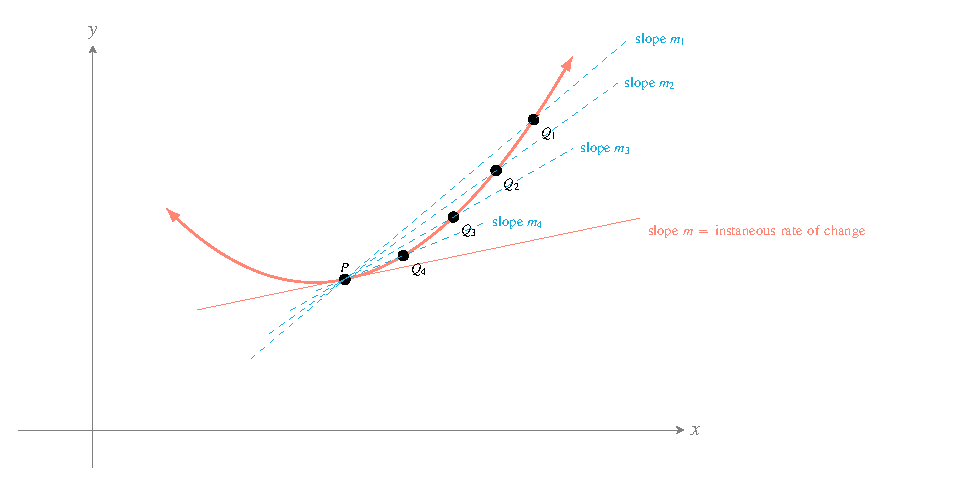
\includegraphics[width=0.8\textwidth]{sec-tan}
\caption{导数的几何意义的来源}
\end{figure}

因此对于任何一个函数$y=f(x)$,其导数的表达式均可通过以下的表达式进行求算:
\[
	\fbox{$f'(x)=\lim\limits_{h\to 0} \frac{f(x+h)-f(x)}{(x+h)-x}$}
\]
这就是之前缺少的一块拼图。
这个表达式求算的就是两个点$\left( x,f(x)\right)$以及$\left( x+h, f(x+h)\right)$连成的直线的斜率\footnote{割线斜率}。当$h\to 0$越来越接近于$0$的时候,就变成了切线的斜率。也就是导数。所以,我们利用该表达式推导了后续其他函数的导数。关于导数的定义,可以参考该\href{https://www.bilibili.com/video/BV1c7411D74J}{视频}了解更多

\subsection*{常见初等函数的导数}
根据导数的定义,我们就再也不需要画切线了,直接通过代数方法求算常见函数的导数。得到以下的结果:\\
\[

\begin{matrix}
 \frac{\d}{\d x}e^x=e^x  & \frac{\d}{\d x}\ln x=\frac{1}{x}\\
 \frac{\d}{\d x}\sin x=\cos x & \frac{\d}{\d x} \cos x=\textcolor{r1}{-}\sin x  \\
 \frac{\d}{\d x}\tan^x=\sec^2 x &\frac{\d}{\d x}\tan^{-1}x=\frac{1}{1+x^2}
\end{matrix}

\]

那么,我们就来用代数表达式证明一下第一个指数函数的导数。
\begin{ExampleBox}
prove the derivative of $f(x)=e^x$ is still $e^x$.
\tcblower
\begin{align*}
  f'(x) &=\lim\limits_{h\to 0} \frac{f(x+h)-f(x)}{(x+h)-x}\\
        &=\lim\limits_{h\to 0}\frac{e^{x+h}-e^x}{x+h-x}\\
        &=\lim\limits_{h\to 0} e^x \cdot \fbox{$\frac{e^h-1}{h}$}\\
        &=e^x \cdot \fbox{$\lim\limits_{h\to 0}\frac{e^h-1}{h}$}\\
        &=e^x
\end{align*}
关于方框当中的部分,是来自于$e$的定义。可以查看\href{https://www.bilibili.com/video/BV15a4y1v74j}{赵三金的视频}1min 05s处。或者查看\href{https://www.bilibili.com/video/BV11x411e7FN}{3Blue1Brown的视频} 7min 44s处,了解更多
\end{ExampleBox}

在上面的$6$个基本函数的导数中,$y=\ln x$以及 $y=\tan^{-1} x$如果从基本定义出发的话,需要利用到$e=\lim\limits_{h\to 0} \left(1+h\right)^{\frac{1}{h}}$,$\tan^{-1} x-\tan^{-1}y =\tan^{-1}\left(\frac{x-y}{1+xy}\right)$以及其他\href{https://www.desmos.com/calculator/sjsgmj4htx}{等价无穷小}的概念。更快的证明方式是通过反函数的导数关系。

\clearpage

\section{导数的求算法则}
在数学世界里并不会处理简单的初等函数。而是这些初等函数通过各种运算构造出的复杂函数。于是就会有如下法则

\subsection*{加减法}
这个是最为简单的处理,如果两个函数直接相加相减,那么导数也直接相加相减就可以了,写成表达式的话的如下:
\[
	f(x)=u(x)\pm v(x)  \qquad f'(x)=u'(x)\pm v'(x)
\]

\subsection*{乘法法则}
这是一个比较重要的求算法则,用于求算,表达式如下:
\[
	f(x) = u(x)\cdot v(x) \qquad \fbox{$f'(x)=u'v + uv'$}
\]
可以查看\href{https://www.bilibili.com/video/BV1Sx411m7Zz}{直观理解链式法则和乘积法则}视频来了解

\subsection*{除法法则}
当两个函数进行相除构造出新的函数的时候,其求算是通过除法法则实现的。表达式和乘法法则有点像,但是也有区别,可以类比地去记忆
\[
	f(x) =\frac{u(x)}{v(x)} \qquad \fbox{$f'(x)=\frac{u'v-uv'}{v^2}$}
\]
比如$y=\tan x$的导数就可以利用除法法则证明
\begin{ExampleBox}
首先要利用\ref{sec:Trig Identity}当中$\tan =\frac{\sin}{\cos}$转变为正弦函数与余弦函数之商的形式,再利用除法法则进行求算

\begin{align*}
  f(x) &= \tan x =\frac{\sin x}{\cos x}=\frac{u}{v}\\
  f'(x)&= \frac{u'v-uv'}{v^2}\\
       &= \frac{\cos x\cdot \cos x- \sin x\cdot (-\sin x)}{\cos^2 x}\\
       &=\frac{\cos^2 x+\sin^2 x}{\cos^2 x}\\
       &=\frac{1}{\cos^2 x}\\
       &=\sec^2 x
\end{align*}
\gls{QED}
\end{ExampleBox}

\begin{TaskBox}
尝试着用导数的定义,推导除法法则:\\
$f'(x)=\lim\limits_{h\to 0}\frac{\frac{u(x)}{v(x+h)}-\frac{u(x)}{v(x)}}{h}$
\end{TaskBox}


\subsection*{链式法则}
链式法则可以说是求导法则当中最重要的一个法则了。利用的是微分的可传递性。为如下的形式:
\begin{align*}
 \frac{\d y}{\d x} &=\frac{\d y}{\d u} \cdot \frac{\d u}{\d x}\\
 \frac{\d }{\d x}f(g(x)) &= f'(\boxed{g(x)})\cdot g'(\boxed{x})
\end{align*}
虽然考试当中常考两层嵌套的函数,但是链式法则的强大之处在于无论是多少层嵌套的复合函数都是可以使用的。

\begin{ExampleBox}
利用链式法则求算$y=a^x$的导数
\tcblower
首先利用$a^x=\left(e^\ln a\right)^x$将该函数视作$y=e^u$与$u=a\cdot \ln a$的复合函数,先做好准备工作$\frac{\d y}{\d u}=e^u$, $\frac{\d u}{\d x}=\ln a$。最后再利用chain rule可以得到:
\[
\frac{\d y}{\d x} =\frac{\d y}{\d u}\cdot \frac{\d u}{\d x} =e^u\cdot \ln a =e^{x\ln a}\cdot \ln a =a^x \cdot \ln a 
\]
\end{ExampleBox}

在\href{https://www.bilibili.com/video/BV1Sx411m7Zz}{直观理解链式法则和乘积法则}这个视频中,可视化地分析了链式法则的基本原理。每一个导数都像一个链节,可以不停地传递下去。因此哪怕复合层数再多也不用怕,区分每一层,然后不停写下去就好了。

\begin{SummBox}
\begin{itemize}
\item 乘法法则:$\frac{\d y}{\d x}=u'v + uv'$
\item 除法法则:$\frac{\d y}{\d x}=\frac{u'v-uv'}{v^2}$
\item 链式法则:$\frac{\d y}{\d x}=\frac{\d y}{\d u}\times \frac{\d u}{\d \ldots}\times \cdots \times \frac{\d \ldots}{\d x}$
\item 请写出常见函数的导数:
\vspace{5 em}
\end{itemize}
\end{SummBox}
\clearpage

\section{参数函数和隐函数导数}
接下来是处理两类特殊的函数的导数。只要掌握固定的求算方法即可。
\subsection*{参数函数导数}
参数函数并没有直接给出因变量和自变量的直接关系,而是通过另外一个的变量,把自变量和因变量联系起来,比如$\begin{cases}
x=f(t)\\
y=g(t)
\end{cases}$通过这样方法定义的表达式就是一个参数函数,本质上$x$与$y$之间依旧满足一一对应的关系的。只不过需要借助一个新的参数$t$。

对于这样的函数,我们可以通过分别求算$\frac{\d x}{\d t}$和$\frac{\d y}{\d t}$。再将这两个导数做商,进而获得$\frac{\d y}{\d x}$的结果,用表达式就是:
\[
	\frac{\d y}{\d x}=\frac{\frac{\d y}{\d t}}{\frac{\d x}{\d t}}
\]
\begin{ExampleBox}
The position of a particle moving in the $xy$-plane is given by $x(t)=t^3-3t^2 , y(t)=12t-3t^2$. Find the expression for the tangent when $t=1$.
\tcblower
带入$t=1$可知此时该点处于$(-2,9)$。因此只需要找出导数,即可利用点斜式$y-9=m(x+2)$表示切线。

分别求算$\frac{\d x}{\d t}=3t^2-6t=-3$,$\frac{\d y}{\d t}=13-6t=6$。即可得到$\frac{\d y}{\d x}=-2$

因此最后切线为 $y-9=-2(x+2)$
可以参考\href{https://www.desmos.com/calculator/sbvuiwhorn}{该desmos}帮助理解。
\end{ExampleBox}

\subsection*{隐函数求导}
对于$x$,$y$出现在一起,且无法分离的函数。一般可以计作$f(x,y)=0$\footnote{把所有含有变量的项全部调整到等于号的左侧就可以得到这样的形式,不移动也没有关系}这样的函数称之为隐函数。处理这种类型的函数,只需要记住两个要点:
\begin{itemize}
	\item $y$是关于$x$的函数,因此$y=f(x)$。虽然写不出具体表达式;
	\item 微分是一种运算手段,因此对等式两边可以同时求算微分\textbf{Differentiating each term with respect to $x$},并且等式关系依旧成立。
\end{itemize}
这样就可以求算了。最后导数的表达式中会同时含有$x$和$y$,但这并不是不被允许的。

\begin{ExampleBox}
Find the derivative of $x^2+3y=6xy$
\tcblower
只要两边同时求导就好了。可以移项,把$6xy$移动到左边;也可以不移动。
\begin{align*}
 \frac{\d}{\d x} \left(x^2+3y\right) &= \frac{\d}{\d x} \left(6xy\right)\\
 2x+3\frac{\d y}{\d x} &=6\cdot \left(1\cdot y + x\cdot \frac{\d y}{\d x}\right)\\
 (3-6x)\frac{\d y}{\d x} &=6y-2x\\
 \frac{\d y}{\d x} &=\frac{6y-2x}{3-6x}
\end{align*}
\end{ExampleBox}

只不过,在这里,容易出错的地方是$\frac{\d xy}{\d x}$其结果要当做是$x\cdot f(x)$这样的两个函数相乘再求导。因此会利用product rule;在其他情况当中也可能需要利用chain rule进行求算。
\begin{TaskBox}
Find the derivative of the implicit function $x^{2}+x\cdot \tan\ y=3$.
\end{TaskBox}